

Na \orig{50} našich příkladech jsme viděli, že u velmi špatně
podmíněných úloh dává i ortogonalizační algoritmus výsledky
znehodnocené zaokrouhlovacími chybami. Přitom z hlediska numerické stability
je např. u ortogonalizace popsané vzorci (2.1) patrně nejcitlivější
krok ($2.1_2$); jak hned ukážeme.

Uvedli jsme již, že je-li některý sloupec $a_i$ ortogonalizované
matice $A$ roven lineární kombinaci předchozích sloupců, pak
odpovídající sloupec $\widetilde w_i$ bude teoreticky
nulový. Analogicky, bude-li sloupec $a_i$, blízký některé lineární
kombinaci předchozích sloupců, budou patrně i prvky sloupce
$\widetilde w_i$ blízké nule. Při numerickém výpočtu podle $2.1_2$
musí potom ovšem dojít ke ztrátě platných cifer složek vektoru
$\widetilde w_i$, který tak bude zkreslen relativně velkou chybou,
stejně jako vektor $w_i$ z něho
odvozený normalizací podle
%
$2.1_3$%
  \footnote{%
%
Při měření relativní chyby vektoru $\widetilde w_i$ můžeme vycházet z
porovnání délek $\Vert a_i\Vert$ a $\Vert\widetilde w_i\Vert$. Tímto jednoduchým
diagnostickým prostředkem můžeme testovat regularitu resp. míru
podmíněnosti řešené úlohy.
%
}.
%
Takto deformovaný vektor$\widetilde w_i$ pak obecně nemusí plně
vyhovovat žádnému ze dvou požadavků, podle nichž byl konstruován:
nemusí splňovat podmínky ortogonality k vektorům $w_j (j<i)$ a nemusí
ležet v prostoru $E_i (a_1, a_2, \dots, a_i)$.
%
Jak se zdá, lze jednoduchým způsobem odstranit
pouze první z uvedených nedostatků postupem, který je z lineární
algebry znám pod pojmem doortogonalizace
%
\footnote{Český termín byl převzat z Fiedlerova překladu [12], kde
  se na str. 277 pojednává o užití takového postupu v~souvislosti s
  metodou konjugovaných směrů pro řešení soustav lineárních
  algebraických rovnic. Na str. 622 téže publikace se užívá
  alternativního termínu ``přeortogonalizace''.
}
%
[30], [38, str. 354].  Věnujme bližší pozornost tomuto postupu.


Mějme soustavu ortonormálních vektorů $w_1,w_2,\dots,w_{i-1}$. K těmto
vektorům budeme Gra\-mo\-vým--Schmidtovým postupem ortogonalizovat
vektor $a_i$.  Nechť $\widetilde w_i$ je vektor vzniklý exaktní
ortogonalizací $a_i$ podle ($2.1_2$). \orig{51} Výsledkem numericky
provedené ortogonalizace je pak vektor $\widetilde w'_i$ zatížený
chybou $\varphi'_i$
%
\begin{align*}
  \tag{6.1}
  {\widetilde w}'_i = \widetilde w_i + \varphi'_i \Punc{.}
\end{align*}
%
Naší snahou bude korigovat vektor $\widetilde w'_i$ tak, aby v
některém smyslu došlo k poklesu chyby $\varphi'_i.$ Předpokládejme
korigovaný vektor $\widetilde w'_i$ ve tvaru
%
\begin{align*}
  \tag{6.2}
  \widetilde w''_i = \widetilde w'_i
  + \sum_{j=1}^{i-1} \alpha_jw_j = \widetilde w'_i + W\alpha
  \Punc{,}
\end{align*}
%
kde $W$ je matice se sloupci $w_j (j=1,2,\dots,i-1)$.  Koeficienty
$\alpha_j$ určíme metodou nejmenších čtverců tak, aby pro odpovídající
chybu $\varphi''_i$ vektoru $\widetilde w''_i$
%
\begin{align*}
  \tag{6.3}
  \varphi''_i = \widetilde w''_i - \widetilde w_i =
  W\alpha + (\widetilde w''_i - \widetilde w_i)  =
  W\alpha + \varphi'_i
\end{align*}
%
byla splněna minimalizační podmínka
%
\begin{align*}
  \tag{6.4}
  (\varphi''_i,\varphi''_i) = \min.
\end{align*}
%
Uvážíme-li, že $W^TW = E$ a $W^T\widetilde w_i = 0$, snadno najdeme,
že
%
\begin{align*}
  \tag{6.5}
  \alpha &= -W^T\widetilde w'_i \\
  \tag{6.6}
  \widetilde w''_i &= \widetilde w'_i - WW^T\widetilde w'_i =
  \widetilde w'_i -
  \sum_{j=1}^{i-1}(\widetilde w'_i,w_j)w_j \Punc{.}
\end{align*}
%
Vzorec (6.6) je formálně stejný jako vzorec ($2.1_2$). pouze s tím
rozdílem, že místo vektoru $a_i$ zaujímá nyní vektor $\widetilde
w'_i$. Vidíme tedy, že \Xemph{korekce vektoru $\widetilde w'_i$,
  založená na požadavku (6.4) spočívá v~opakované ortogonalizaci, při
  níž vektor $\widetilde w'_i$ získaný ortogonalizací $a_i$, znovu
  ortogonalizujeme k vektorům $w_j (j=1,2,\dots,i-1)$}.


Jsou-li koeficienty $\alpha_j$ určeny podle (6.5), pak lze dokázat,
že pro chybu $\varphi_i''$ platí
%
\begin{align*}
  \tag{6.7}
  \Vert\varphi_i''\Vert^2 =
  \Vert\varphi_i'\Vert^2 - \Vert\alpha\Vert^2 \le \Vert\varphi_i'\Vert^2 \Punc{.}
\end{align*}
%
Přínos \orig{52} doortogonalizace závisí tedy na velikosti skalárního
součinu $\Vert\alpha\Vert^2$. Dokážeme, že tento součin může v některých
příznivých případech dosáhnout hodnoty až $\Vert\varphi_i'\Vert^2$ a tak
anulovat chybu $\varphi_i''$.


\Xemph{Věta 1. Leží-li vektor chyby $\varphi_i'$ v prostoru $E_i$
  vytvářeném ortonormálními vektory $w_1,w_2,\dots,w_i$, pak přínos
  doortogonalizace je maximální. Odpovídající chyba $\varphi_i''$
  korigovaného vektoru $\widetilde w''_i$ je po jeho normalizaci
  nulová}.
%
Věta platí za předpokladu, že vektor $\widetilde w''_i$ je
nenulový.

Důkaz: leží-li $\varphi'$ v $E_i$, pak lze psát
%
\begin{align*}
  \tag{6.8}
  \varphi' = \sum_{j=1}^i \beta)_j w_j \Punc{,}
\end{align*}
%
kde $\beta_j$ jsou reálné koeficienty. Hledáme opět vektor $\alpha$,
který minimalizuje odpovídající veličinu $(\varphi''_i,
\varphi''_i)$.
%

\noindent Položme
\begin{align*}
  \tag{6.9}
  \beta = (\beta_1,\beta_2,\dots,\beta_{i-1})^T,
  \qquad\alpha = -\beta \Punc{.}
\end{align*}
%
Potom je podle (6.3) a (6.8)
\begin{align*}
  \tag{6.10}
  \varphi_i'' &= -W\beta + \varphi_i'
  = -W\beta + W\beta + \beta_iw_i - \beta_iw) \Punc{,}\\
  \widetilde w_i'' &= \widetilde w_i + \varphi_i'' =
  (\Vert \widetilde w_i\Vert + \beta_)w_i \Punc{.}
\end{align*}
%
Za předpokladu,že $\widetilde w_i'' \ne 0$, dostaneme po
normalizaci
%
\begin{align*}
  \tag{6.11}
  \widetilde w_i''/\Vert w_i''\Vert =
  (\widetilde w_i + \beta_i)(| \Vert\widetilde w_i\Vert + \beta_i|)^{-1}w_i
  = tw_i \Punc{.}
\end{align*}
%
Uvážíme-li, že při ortogonalizačním procesu mohou být znaménka
normalizovaných vektorů volena libovolně (kap. 2), pak (6.11)
dokazuje, že vektor $\widetilde w''_i$ splyne po normalizaci s
hledaným vektorem $w_i$. Věta 1 tedy platí. Z dokázané věty plyne
mj. zajíma- vý závěr, že doortogonalizace přináší maximální užitek při
případné ortogonalizaci $m$-tého a dalších sloupců matice o $m$
řádcích.

Vedle případů, kdy doortogonalizace podstatně zvýší přesnost
ortogonalizačního procesu, existují ovšem i případy, kdy chyba
ortogonalizovaného vektoru doortogonalizací neklesne. Stane se
%
tak \orig{53} v případě, bude-lí vektor chyby $\varphi_i'$
ortogonální k vektorům $w_1,w_2,\dots,w_{i-1}$.  Potom totiž ze (6.5)
a (6,1) plyne
%
\begin{align*}
  \tag{6.12}
  \alpha  = -W^T(\widetilde w_i + \varphi_i')
  = W^T\varphi_i' = 0 \Punc{,}
\end{align*}
%
takže podle (6.3) bude skutečně $\varphi_i'' = \varphi_i'$.


%%% { \input{doortogonalizace2} } %%%
%%%
%%% \newcommand{\OA}  {\ensuremath{(\overrightarrow{\mathrm{OA}})}}
%%% \newcommand{\OW}  {\ensuremath{(\overrightarrow{\mathrm{O%
%%%         \widetilde W}}\,')}}
%%% \newcommand{\OWi} {\ensuremath{(\overrightarrow{\mathrm{O%
%%%         \widetilde W}})}}
%%% \newcommand{\OWii}{\ensuremath{(\overrightarrow{\mathrm{O%
%%%         \widetilde W}}\,'')}}


Pro větší názornost budeme myšlenku doortogonalizace graficky
ilustrovat příkladem ortogonalizace vektoru
%
$ \underline a$ ~ \OA ~ k vektoru $w_1$
%
v trojrozměrném prostoru. V souladu se zavedenou symbolikou budeme
značit

\vspace{1ex}
\begin{tabularx}{\textwidth}{llcX}%
  $\widetilde w$ & \OW & - &
  %
  vektor získaný přesnou ortogonaiizací vektoru $\underline a$
  k vektoru $w_1$, \\
  %
  $\widetilde w\,'$ & \OWi & - &
  %
  vektor získaný přibližnou ortogoralizací (s chybou $\varphi\,'$)
  $\underline a$ k $w_1$,\\
  %
  $\widetilde w\,''$ & \OWii & - &
  vektor korigovaný doortogonalizací,\\
  %
  $\varphi\,''$ & ~ & - &
  chybu doortogonalizovaného vektoru $\widetilde w\,''$.\\
\end{tabularx}\\[1ex]

\noindent
Obr. 6.1 naznačuje princip doortogonalizace, obrázky 6.2 a 6.3
ilustrují extrémní případy maximálního a minimálního přínosu
doortogonalizace. Na všech obrázcích značí $\pi_1$, rovinu kolmou k
$w_1$ a $\pi_2$ rovinu obsahující vektory $w_1$, $\underline{a}$ a
tedy tedy i $\widetilde w$. Rovnice (2.1) resp. (6.6) aplikované na
náš příklad vedou k následující jednoduché geometrické konstrukci
ortogonalizovaného resp. doortogonalizovaného vektoru $\widetilde w$
resp. $\widetilde w\,''$: ~bodem $A$ resp.  $\widetilde W\,'$ stačí
sestrojit rovnoběžku s $w_1$ a najít její průsečík s rovinou $\pi_1$.

\orig{54}

\begin{figure}\centering
%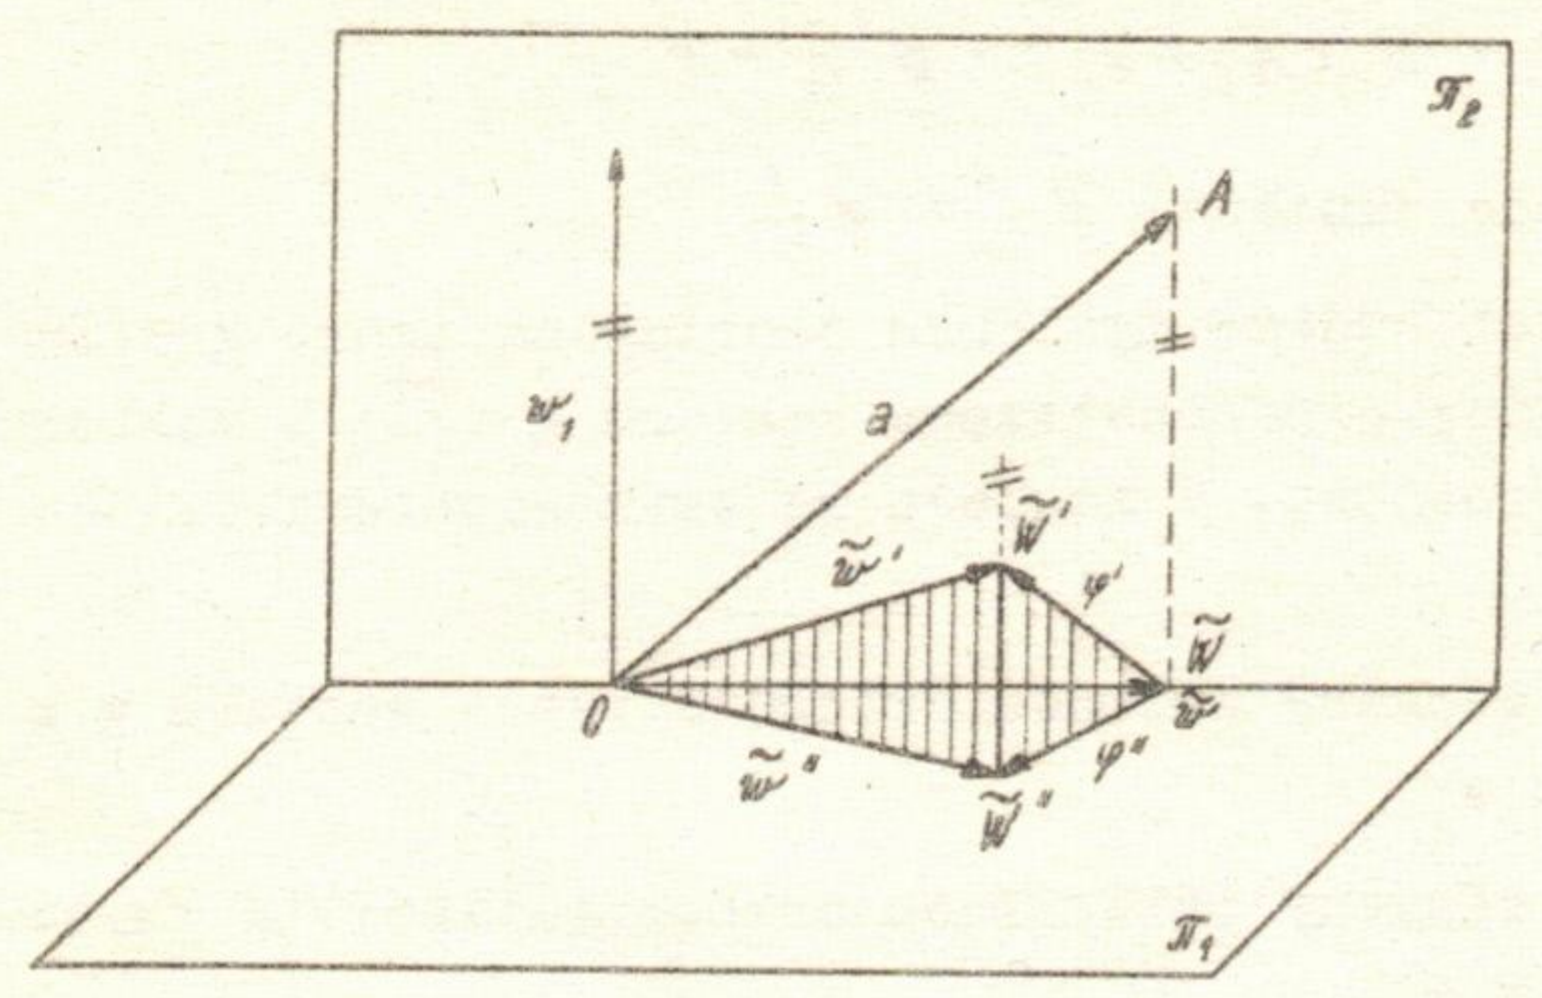
\includegraphics[width=0.75\textwidth]{obr_6.1.png}
% digitalizace https://yangcha.github.io/iview/iview.html
%
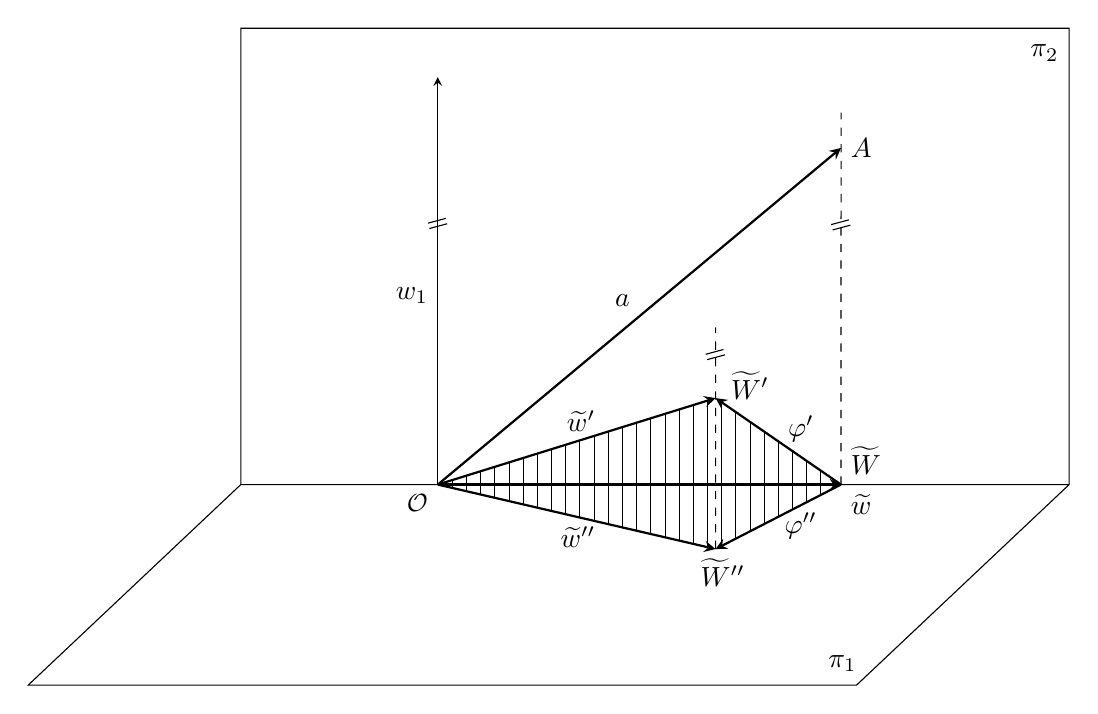
\begin{tikzpicture}[xscale=9,yscale=-9,>=stealth]

  \begin{scope}   % projekcni roviny pi_1 a pi_2

    \def\Mx{0.331};
    \def\My{0.684};
    \coordinate(M) at (\Mx,\My);
    \def\Nx{1.500};
    \def\Ny{\My};
    \coordinate(N) at (\Nx,\Ny);
    \def\Px{\Nx};
    \def\Py{0.040};
    \coordinate(P) at (\Px,\Py);
    \def\Rx{\Mx-0.300};
    \def\Ry{0.967};
    \coordinate(R) at (\Rx,\Ry);
    \def\Qx{\Mx};
    \def\Qy{\Py};
    \coordinate(Q) at (\Qx,\Qy);
    \def\Sx{\Nx-0.300};
    \def\Sy{\Ry};
    \coordinate(S) at (\Sx,\Sy);

    \draw[thin] (M)--(N)--(P)--(Q)--(M)--(R)--(S)--(N);

    \node at (\Px - 0.035,\Py + 0.035) {$\pi_2$};
    \node at (\Sx - 0.020,\Sy - 0.030) {$\pi_1$};

    \def\Ox{0.609};
    \def\Oy{\My};
    \coordinate (O) at (\Ox,\Oy);
    \node at (O) [below left] {{\small $\mathcal{O}$}};

    \def\Ax{1.178};
    \def\Ay{0.209};
    \coordinate (A) at (\Ax,\Ay);
    \def\Bx{\Ax};
    \def\By{\My};
    \coordinate (B) at (\Bx,\By);
    \def\Cx{1.001};
    \def\Cy{0.775};
    \coordinate (C) at (\Cx,\Cy);
    \def\Dx{\Cx};
    \def\Dy{0.562};
    \coordinate (D) at (\Dx,\Dy);

    \def\Ex{\Ox};
    \def\Ey{\Ay-0.100};
    \coordinate (E) at (\Ex,\Ey);
    \draw[ ->] (O)--(E);
    \node at (\Ex,0.417) [left] {$w_1$};
    \node at (\Ex,0.317) {\rotatebox{15}{$\overline{\overline{~~}}$}};

    \draw[thick, ->] (O)--(A);
    \draw[thick, ->] (O)--(B);
    \draw[thick, ->] (O)--(C);
    \draw[thick, ->] (O)--(D);
    \draw[thick, ->] (B)--(C);
    \draw[thick, ->] (B)--(D);

    \node at (A) [right] {$A$};

    \draw[thin, dashed] (B)--(\Ax,\Ay-0.050);
    \node at (\Ax,\Ay+0.110) {\rotatebox{15}{$\overline{\overline{~~}}$}};
    \draw[thin, dashed] (C)--(\Dx,\Dy-0.100);
    \node at (\Dx,\Dy-0.060) {\rotatebox{15}{$\overline{\overline{~~}}$}};

    \node[above left ] at ({(\Ox+\Ax)/2},{(\Oy+\Ay)/2}) {$a$};
    \node[above right] at (B) {$\widetilde W$};
    \node[below right] at (B) {$\widetilde w$};
    \node[below right] at ({(\Bx+\Cx)/2-0.005},{(\By+\Cy)/2-0.020})
         {$\varphi''$};
    \node[below] at (\Cx+0.010,\Cy) {$\widetilde W''$};
    \node[below left ] at({(\Ox+\Cx)/2+0.040},{(\Oy+\Cy)/2})
         {$\widetilde w''$};
    \node[above left ] at({(\Ox+\Dx)/2+0.040},{(\Oy+\Dy)/2})
         {$\widetilde w'$};
    \node[above right] at({\Dx+0.008},{\Dy+0.015}) {$\widetilde W'$};
    \node[below right] at ({(\Bx+\Dx)/2},{(\By+\Dy)/2-0.050})
         {$\varphi'$};

     \clip (O)--(C)--(B)--(D)--cycle;
     \foreach \i in {0,...,30}
     {
        \def\dx{0.02*\i};
        \draw[ultra thin] (\Ox + \dx,\Cy+0.1)--(\Ox + \dx,\Dy-0.2);
     }

  \end{scope}

\end{tikzpicture}

%

%
\label{6.1.}
\caption{Princip doortogonalizace -- vektor chyby $\varphi'$ má
obecnou polohu vzhledem k $\pi_1$ a $\pi_2$
$(\Vert\varphi''\Vert < \Vert\varphi'\Vert)$.}
%
\end{figure}

\begin{figure}\centering
%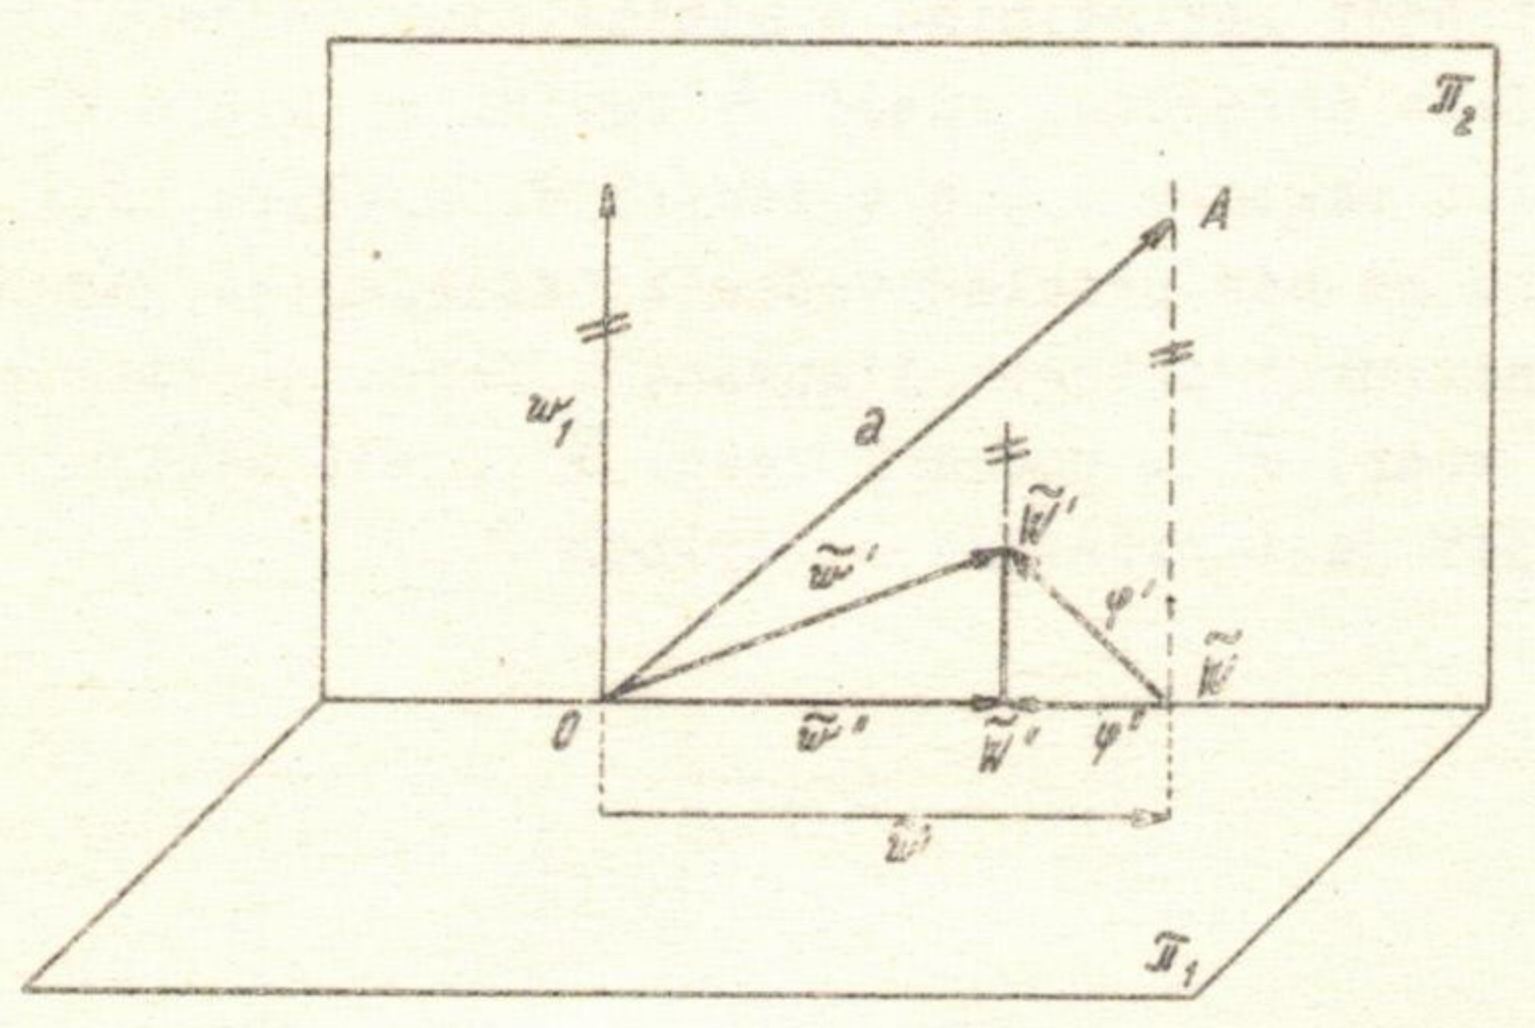
\includegraphics[width=0.75\textwidth]{obr_6.2.png}
% digitalizace https://yangcha.github.io/iview/iview.html
%
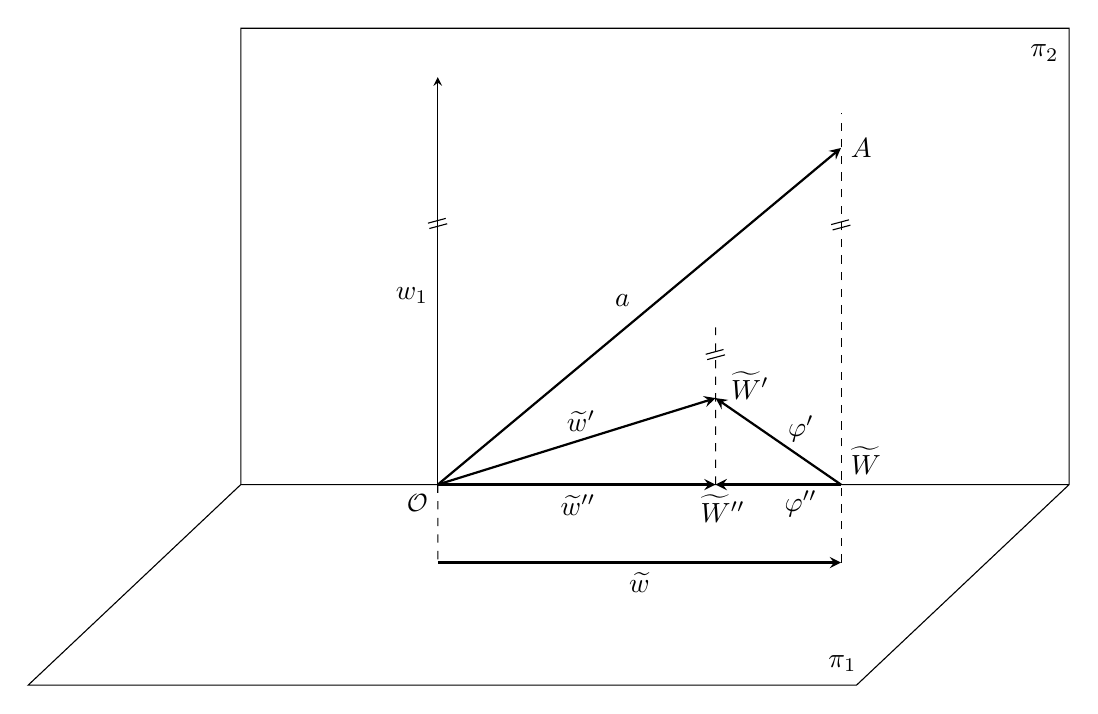
\begin{tikzpicture}[xscale=9,yscale=-9,>=stealth]

  \begin{scope}   % projekcni roviny pi_1 a pi_2

    \def\Mx{0.331};
    \def\My{0.684};
    \coordinate(M) at (\Mx,\My);
    \def\Nx{1.500};
    \def\Ny{\My};
    \coordinate(N) at (\Nx,\Ny);
    \def\Px{\Nx};
    \def\Py{0.040};
    \coordinate(P) at (\Px,\Py);
    \def\Rx{\Mx-0.300};
    \def\Ry{0.967};
    \coordinate(R) at (\Rx,\Ry);
    \def\Qx{\Mx};
    \def\Qy{\Py};
    \coordinate(Q) at (\Qx,\Qy);
    \def\Sx{\Nx-0.300};
    \def\Sy{\Ry};
    \coordinate(S) at (\Sx,\Sy);

    \def\Ty{0.110};   % odsazeni vektoru \widetilde w pod osou O-B

    \draw[thin] (M)--(N)--(P)--(Q)--(M)--(R)--(S)--(N);

    \node at (\Px - 0.035,\Py + 0.035) {$\pi_2$};
    \node at (\Sx - 0.020,\Sy - 0.030) {$\pi_1$};

    \def\Ox{0.609};
    \def\Oy{\My};
    \coordinate (O) at (\Ox,\Oy);
    \node at (O) [below left] {{\small $\mathcal{O}$}};

    \def\Ax{1.178};
    \def\Ay{0.209};
    \coordinate (A) at (\Ax,\Ay);
    \def\Bx{\Ax};
    \def\By{\My};
    \coordinate (B) at (\Bx,\By);
    \def\Cx{1.001};
    %%%\def\Cy{0.775};   obr 6.1
    \def\Cy{\Oy};
    \coordinate (C) at (\Cx,\Cy);
    \def\Dx{\Cx};
    \def\Dy{0.562};
    \coordinate (D) at (\Dx,\Dy);

    \def\Ex{\Ox};
    \def\Ey{\Ay-0.100};
    \coordinate (E) at (\Ex,\Ey);
    \draw[ ->] (O)--(E);
    \node at (\Ex,0.417) [left] {$w_1$};
    \node at (\Ex,0.317) {\rotatebox{15}{$\overline{\overline{~~}}$}};

    \draw[thick, ->] (O)--(A);
    %%%\draw[thick, ->] (O)--(B);   obr 6.1
    \draw[thick, ->] (O)--(C);
    \draw[thick, ->] (O)--(D);
    \draw[thick, ->] (B)--(C);
    \draw[thick, ->] (B)--(D);

    \node at (A) [right] {$A$};

    \draw[thin, dashed] (\Bx,\By+\Ty)--(\Ax,\Ay-0.050);
    \node at (\Ax,\Ay+0.110) {\rotatebox{15}{$\overline{\overline{~~}}$}};
    \draw[thin, dashed] (C)--(\Dx,\Dy-0.100);
    \node at (\Dx,\Dy-0.060) {\rotatebox{15}{$\overline{\overline{~~}}$}};

    \node[above left ] at ({(\Ox+\Ax)/2},{(\Oy+\Ay)/2}) {$a$};
    \node[above right] at (B) {$\widetilde W$};
    \node[below right] at ({(\Bx+\Cx)/2-0.005},{(\By+\Cy)/2-0.005})
         {$\varphi''$};
    \node[below] at (\Cx+0.010,\Cy) {$\widetilde W''$};
    \node[below left ] at({(\Ox+\Cx)/2+0.040},{(\Oy+\Cy)/2})
         {$\widetilde w''$};
    \node[above left ] at({(\Ox+\Dx)/2+0.040},{(\Oy+\Dy)/2})
         {$\widetilde w'$};
    \node[above right] at({\Dx+0.008},{\Dy+0.015}) {$\widetilde W'$};
    \node[below right] at ({(\Bx+\Dx)/2},{(\By+\Dy)/2-0.050})
         {$\varphi'$};

     %%%\clip (O)--(C)--(B)--(D)--cycle;    obr 6.1
     %%%\foreach \i in {0,...,30}
     %%%{
     %%%   \def\dx{0.02*\i};
     %%%   \draw[ultra thin] (\Ox + \dx,\Cy+0.1)--(\Ox + \dx,\Dy-0.2);
     %%%}

    \draw[dashed] (O)--(\Ox,\Oy+\Ty);
    \draw[thick, ->] (\Ox,{\Oy+\Ty})--(\Bx,\By+\Ty);
    \node[below] at ({(\Ox+\Bx)/2},{\Oy+\Ty}) {$\widetilde w$};

  \end{scope}

\end{tikzpicture}

%

%
\label{6.2.}
\caption{Maximální přínos doortogonalizace -- vektor $\varphi'$ leží
  v rovině $\pi_2$ (normalizací $\widetilde w\,''$ se chyba
  $\varphi'$ anuluje).}
%
\end{figure}

\begin{figure}\centering
%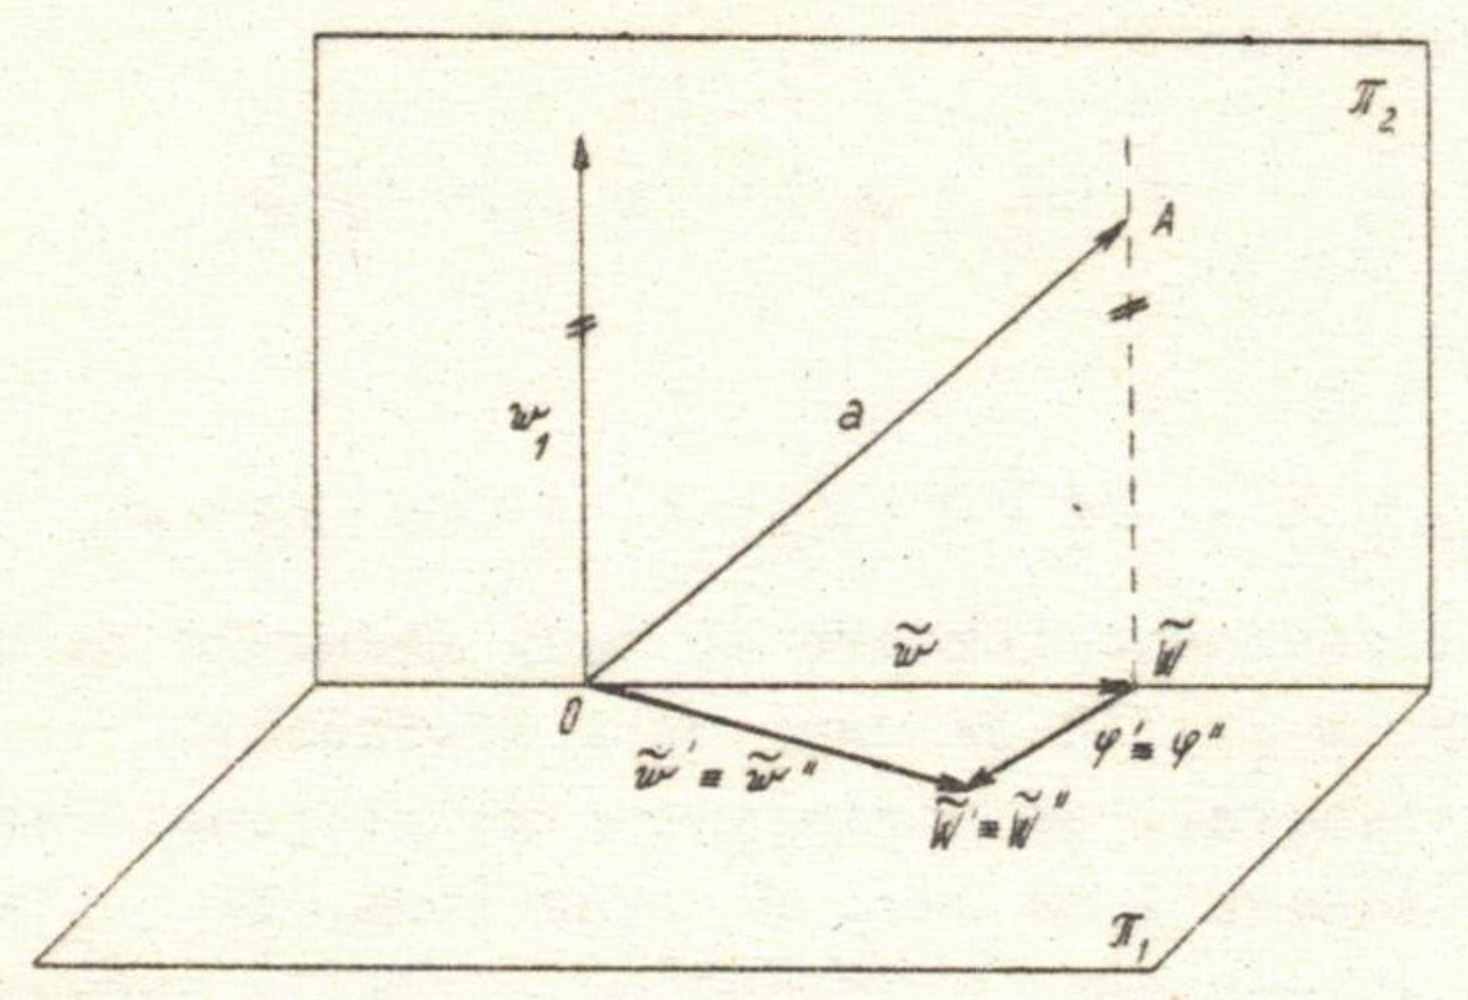
\includegraphics[width=0.75\textwidth]{obr_6.3.png}
% digitalizace https://yangcha.github.io/iview/iview.html
%
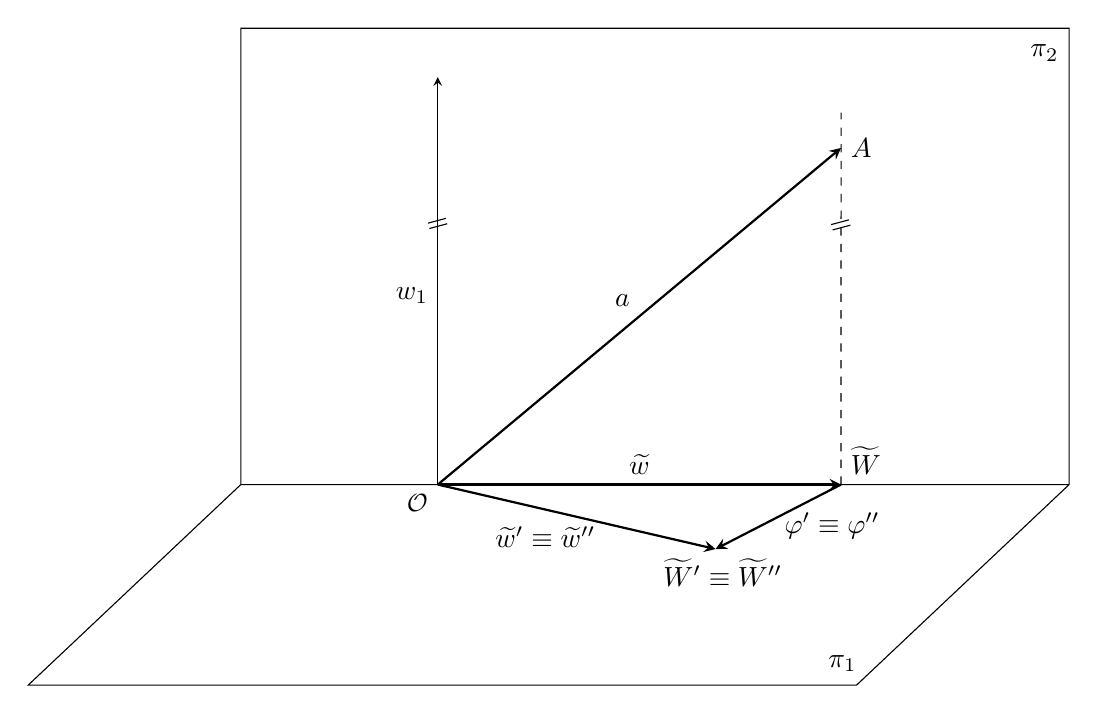
\begin{tikzpicture}[xscale=9,yscale=-9,>=stealth]

  \begin{scope}   % projekcni roviny pi_1 a pi_2

    \def\Mx{0.331};
    \def\My{0.684};
    \coordinate(M) at (\Mx,\My);
    \def\Nx{1.500};
    \def\Ny{\My};
    \coordinate(N) at (\Nx,\Ny);
    \def\Px{\Nx};
    \def\Py{0.040};
    \coordinate(P) at (\Px,\Py);
    \def\Rx{\Mx-0.300};
    \def\Ry{0.967};
    \coordinate(R) at (\Rx,\Ry);
    \def\Qx{\Mx};
    \def\Qy{\Py};
    \coordinate(Q) at (\Qx,\Qy);
    \def\Sx{\Nx-0.300};
    \def\Sy{\Ry};
    \coordinate(S) at (\Sx,\Sy);

    \draw[thin] (M)--(N)--(P)--(Q)--(M)--(R)--(S)--(N);

    \node at (\Px - 0.035,\Py + 0.035) {$\pi_2$};
    \node at (\Sx - 0.020,\Sy - 0.030) {$\pi_1$};

    \def\Ox{0.609};
    \def\Oy{\My};
    \coordinate (O) at (\Ox,\Oy);
    \node at (O) [below left] {{\small $\mathcal{O}$}};

    \def\Ax{1.178};
    \def\Ay{0.209};
    \coordinate (A) at (\Ax,\Ay);
    \def\Bx{\Ax};
    \def\By{\My};
    \coordinate (B) at (\Bx,\By);
    \def\Cx{1.001};
    \def\Cy{0.775};
    \coordinate (C) at (\Cx,\Cy);
    %%%\def\Dx{\Cx};    obr 6.1
    %%%\def\Dy{0.562};
    %%%\coordinate (D) at (\Dx,\Dy);

    \def\Ex{\Ox};
    \def\Ey{\Ay-0.100};
    \coordinate (E) at (\Ex,\Ey);
    \draw[ ->] (O)--(E);
    \node at (\Ex,0.417) [left] {$w_1$};
    \node at (\Ex,0.317) {\rotatebox{15}{$\overline{\overline{~~}}$}};

    \draw[thick, ->] (O)--(A);
    \draw[thick, ->] (O)--(B);
    \draw[thick, ->] (O)--(C);
    %%%\draw[thick, ->] (O)--(D);   obr 6.1
    \draw[thick, ->] (B)--(C);
    %%%\draw[thick, ->] (B)--(D);   obr 6.1

    \node at (A) [right] {$A$};

    \draw[thin, dashed] (B)--(\Ax,\Ay-0.050);
    \node at (\Ax,\Ay+0.110) {\rotatebox{15}{$\overline{\overline{~~}}$}};
    %%%\draw[thin, dashed] (C)--(\Dx,\Dy-0.100);   obr 6.1
    %%%\node at (\Dx,\Dy-0.060) {\rotatebox{15}{$\overline{\overline{~~}}$}};

    \node[above left ] at ({(\Ox+\Ax)/2},{(\Oy+\Ay)/2}) {$a$};
    \node[above right] at (B) {$\widetilde W$};
    %%%\node[below right] at (B) {$\widetilde w$}; obr 6.1
    \node[above] at ({(\Ox+\Bx)/2},{(\Oy+\By)/2}) {$\widetilde w$};
    \node[below right] at ({(\Bx+\Cx)/2-0.005},{(\By+\Cy)/2-0.020})
         {$\varphi'\equiv\varphi''$};
    \node[below] at (\Cx+0.010,\Cy) {$\widetilde W'\equiv\widetilde W''$};
    \node[below left ] at({(\Ox+\Cx)/2+0.040},{(\Oy+\Cy)/2})
         {$\widetilde w'\equiv\widetilde w''$};
    %%%\node[above left ] at({(\Ox+\Dx)/2+0.040},{(\Oy+\Dy)/2})   obr 6.1
    %%%     {$\widetilde w'$};
    %%%\node[above right] at({\Dx+0.008},{\Dy+0.015}) {$\widetilde W'$};
    %%%\node[below right] at ({(\Bx+\Dx)/2},{(\By+\Dy)/2-0.050})
    %%%     {$\varphi'$};

     %%%\clip (O)--(C)--(B)--(D)--cycle; obr 6.1
     %%%\foreach \i in {0,...,30}
     %%%{
     %%%   \def\dx{0.02*\i};
     %%%   \draw[ultra thin] (\Ox + \dx,\Cy+0.1)--(\Ox + \dx,\Dy-0.2);
     %%%}

  \end{scope}

\end{tikzpicture}

%

%
\label{6.3.}
\caption{Minimální přínos doortogonalizace -- vektor $\varphi'$ leží
v rovině $\pi_1$ $(\varphi'' = \varphi')$.}
%
\end{figure}

\noindent
Na obrázcích \orig{55} lze rovněž názorně ilustrovat vzorec (6.7). V
aplikaci např. na obr. 6.1 představuje (6.7) \Xemph{pythagorovu}
větu v~trojúhelníku $\widetilde W\,' \widetilde W\,'' \widetilde W $.

Geometrická představa nás bezprostřeině vede k formulaci následující
důležité věty.

\Xemph{Věta 2. Nechť $E_m$ je prostor, jehož bázi tvoří vektory
  $w_1,w_2,\dots,w_m$.  Označme $\varphi_{i1}$ ortogonální projekci
  chyby $\varphi_i\,'$ vektoru $\widetilde w_i\,'$ $(l<i\le m)$ na
  podprostor $E_{i-l}$ s bází $w_1,w_2,\dots,e_{i-l}$.  Pak při
  doortogonalizaci vektoru $\widetilde w_i\,'$ bude eliminována tato
  složka chyby $\varphi_{i1}$.}

Důkaz. Podle [12, str. 39] lze vektor $\varphi_i\,'$ rozložit na součet
dvou ortogonálních projekcí
%
\begin{align*}
  \tag{6.13}
  \varphi_i\,' = \varphi_{i1} + \varphi_{i2} \Punc{,}
\end{align*}
%
kde $\varphi_{i1}$ je projekce vektoru $\varphi_i\,'$
na $E_{i-l}$ a $\varphi_{i2}$ je projekce  $\varphi_i$
na ortogonální doplněk $E_{i-l}$ Označíme-li $W$ matici se sloupci
$w_1,2_2,\dots,w_{i-l}$, platí tedy
%
\begin{align*}
  \tag{6.14}
  \varphi_{i1} = W\beta, \qquad W^T\!\varphi_{i2} = 0 \Punc{,}
\end{align*}
%
kde \orig{56} vektor $\beta$ je tvořen reálnými koeficienty $\beta_j$
$(j=1,2,\dots,i-l)$.  Podle (6.5) a 160.1) bude potom
%
\begin{align*}
  \tag{6.15}
  \alpha = - W^T\widetilde w_i\,'
  = -W^T(\widetilde w_i + \varphi_i\,'
  = -W^T\varphi_i\,' = -W^T\varphi_{i1}
\end{align*}
%
a po dosazení do (6.3)
%
\begin{align*}
  \tag{6.16}
  \varphi_i\,'' = -WW^T \varphi_{i1} + \varphi_i\,'
  = - WW^TW\beta + \varphi_{i1} + \varphi_{i2}
  = -W\beta + W\beta + \varphi_{i2} = \varphi_{i2} \Punc{.}
\end{align*}
%
Chyba $\varphi_i\,''$ doortogonalizovaného vektoru se tedy redukuje na
složku $\varphi_{i2}$ výchozí chyby $\varphi_i\,'$. Tím je naše věta
dokázána.

Ve větě 2 jsme abstrahovali od normalizace doortogonalizovaného
vektoru $\widetilde w_i\,''$.  V poznámce~1 na str.~\label{LX}
ukazujeme, že při normalizaci je přibližně eliminována ortogonální
projekce zbývající chyby $\varphi_{i2}$ na vektor $w_i$.





Doortogonalizace tedy v obecném případě zpravidla přinese určité
zpřesnění ortogonalizačního procesu, nemusí však tomu tak být
vždy. Stejný závěr platí i pro zobecněnou ortogonalizaci a její
aplikaci při vyrovnání zprostředkujících nebo podmínkových
pozorování. Jiná situace ovšem nastává u zbývajících dvou základních
vyrovnávacích úloh. Vrátíme-li se k závěrům kap. 5 zjišťujeme, že
podle věty 2 \Xemph{doortogonalizace eliminuje právě ty složky chyb,
  které způsobovaly numerickou nestabilitu při řešení úloh typu IC a
  CU ortoconalizací ve spojení se \name{SCHMIDOVÝM} principem
  extremálních vah.} Podívejme se znovu na numerickou stránku
procesu. V kap. 5 jsme uvedli, že po ukončené ortogonalizaci jsou
prvky vektoru $\widetilde w_{A2}$ (horní část $\widetilde w_2$) řádu
\Ocal{10^0} s chybou řádu \Ocal{\delta}.
%
Viděli jsme dále, že očekávaná chyba prvků vektoru $\widetilde w_{B2}$
(spodní část $\widetilde w_2$) je řádu \Ocal{\pi\delta}, přičemž pro
dostatečně velká $\pi$ bude stejného řádu i velikost prvků tohoto
vektoru.  Aplikujeme-li na vektor $\widetilde w_2$ doortogonalizaci,
pak zřejmě při dostatečně velkém $\pi$ dostaneme v horní části
doortogonalizovanéno vektoru nezměněné prvky řádu \Ocal{10^0}, ve
spodní části pak prvky řádu \Ocal{\pi\delta^2} s chybou
\Ocal{\pi\delta^2}.  Úvahu o přínosu doortogonaliizace je možno
opakovat a dalšími doortogonalizacemi postupně snižovat chybu prvků
vektoru $\widetilde w_{B2}$. Vzhledem k očekávanému řádu
\Ocal{\pi^{-1}} těchto prvků by takový proces pokračoval tak dlouho,
pokud by řád chyby doortogonalizovaného vektoru neklesl minimálně
%
%
%
na hodnotu \orig{57} \Ocal{\pi^{-1}\delta}. Jednoduchý výpočet
ukazuje, že potřebný počet $\underline{s}$ doortogonalizací by byl
přibližně roven $s = 2 \log_{10} \pi / log_{10} \delta^{-1}\!$. Např.
pro $\pi = 10^{12}$ a $\delta = 10^{-8}$ je $s=3$. Naznačený
postup je sice názorný a nevyžaduje podstatných úprav
základního ortogonalizačního algoritmu, současně je však zbytečně
zdlouhavý, zejména při velkých hodnotách $\pi$. Popíšeme proto
jednoduchou modifikaci algoritmu, při níž vystačíme ve všech
případech pouze s jedinou doortogonalizací.



Ortogonalizujme sloupec $a_2$ matice $A_{02}$ (5.11) stejným způsobem
jako prve s výsledkem
%
$\widetilde w_ =
\begin{bmatrix}
  \widetilde W_{A2} \\ \widetilde W_{B2}
\end{bmatrix}${.}
%
Základní princip zkráceného doortogonalizačního postupu spočívá v tom,
že dříve než \Xemph{přikročíme k doortogonalizaci vynulujeme prvky
  vektoru} $\widetilde w_{B2}$. Tím se dopouštíme chyby ve spodní
části $\widetilde w_2\;$ \Ocal{\pi^{-1}}, který je pro dostatečně velká
$\pi$ podstatně menší než řád chyby \Ocal{\pi\delta}
odpovídající původnímu postupu. Jediná doortogonalizace vektoru
%
$\begin{bmatrix} \widetilde w_{A2} \\ 0  \end{bmatrix}$
%
potom koriguje jeho chybu s přesností řádově stejnou jako
posloupnost $\underline s$ běžných doortogonalizací vektoru
%
$\widetilde w_2$\,.




Uvedeme ještě poslední modifikaci algoritmu, která má značný
praktický význam, jak se ukáže v následující kapitole. Při
řešení úloh IC a CU jsme až dosud předpokládali, že matice $B$ ve
(5.10) byla "vážena“, tj. explicitně násobena dostatečně velkou
konstantou $\pi$. Při ortogonalizaci resp. doortogonalizaci jsme
pak viděli, že v důsledku toho nebyly potřebné skalární součiny
a normalizační faktory fakticky počítány ze všech prvků
odpovídajících vektorů, ale pouze z prvků jejich některých částí.

Např.  při ortogonalizaci matice $A_{01}$ (5.11) se při vytváření
skalárních součinů neuplatnily prvky matice $A_1$. Zkusíme nyní
modifikovat ortogonalizační algoritmus tak, že \Xemph{budeme
  respektovat naznačené důsledky extrémně velké hodnoty $\pi$, přičemž
  vlastní násobení matice $B$ konstantou $\pi$ explicitně provádět
  nebudeme.}
Ve spojení s výsledky předchozích úvah nás tento orincip vede k
formulaci obecného algoritmu nazvaného ORTON, pomocí něhož bude možno
řešit všechny čtyři kategorie vyrovnávacích úloh.




Mějme blokovou matici
%
\def\TikzBlock#1#2#3#4{%[3]{%
  %\draw (#1*\dx, #2*\dy) rectangle (2, 3)
  \draw (#1,#2) rectangle ((#1+\dx),(#2+\dy));
}
%
\orig{58}
%
\begin{align*}
  \tag{6.17}
  A = \vcenter{\hbox{
  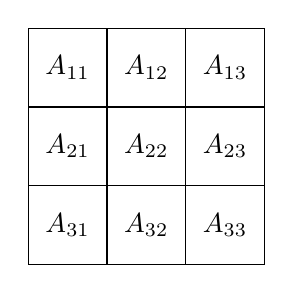
\begin{tikzpicture}[x=1cm,y=1cm]
    \draw (0,2) rectangle (1,3); \draw(0.5,2.5) node{$A_{11}$};
    \draw (1,2) rectangle (2,3); \draw(1.5,2.5) node{$A_{12}$};
    \draw (2,2) rectangle (3,3); \draw(2.5,2.5) node{$A_{13}$};
    \draw (0,1) rectangle (1,2); \draw(0.5,1.5) node{$A_{21}$};
    \draw (1,1) rectangle (2,2); \draw(1.5,1.5) node{$A_{22}$};
    \draw (2,1) rectangle (3,2); \draw(2.5,1.5) node{$A_{23}$};
    \draw (0,0) rectangle (1,1); \draw(0.5,0.5) node{$A_{31}$};
    \draw (1,0) rectangle (2,1); \draw(1.5,0.5) node{$A_{32}$};
    \draw (2,0) rectangle (3,1); \draw(2.5,0.5) node{$A_{33}$};
  \end{tikzpicture} }} \Punc{,}
\end{align*}
%
kde $A_{21}$ je čtvercová regulární matice. Sloupce matice
%
$
\begin{bmatrix}
  A_{11} & A_{12} \\ A_{21} & A_{22}
\end{bmatrix}
$
%
nechť jsou lineárně nezávislé. Algoritmus ORTON lze potom v
podstatě definovat jako posloupnost tří zobecněných ortogonalizací
na vhodně vymezených maticích s cílem určitým způsobem přetvořit
matici $A$ na matici $W$ o stejné blokové struktuře. Přitom první a
třetí ortogonalizace jsou úplné, tj. mají standardní formu
definovanou v kap. 2. Druhá ortogonalizace se uplatní jen v jisté
redukované podobě. Algoritmus ORTON probíhá v následujících krocích:

\begin{enumerate}

\item \Xemph{Zobecněná ortogonalizace matice $A$ se základní maticí
  $A_{21}$, podle schematu}

  \begin{align*}
    \tag{6.18}
    \vcenter{\hbox{
      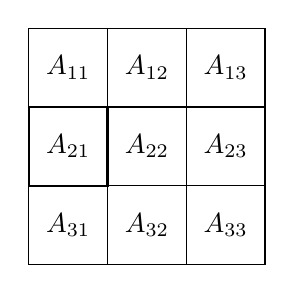
\begin{tikzpicture}[x=1cm,y=1cm]
    \draw (0,2) rectangle (1,3); \draw(0.5,2.5) node{$A_{11}$};
    \draw (1,2) rectangle (2,3); \draw(1.5,2.5) node{$A_{12}$};
    \draw (2,2) rectangle (3,3); \draw(2.5,2.5) node{$A_{13}$};
    \draw[thick]
          (0,1) rectangle (1,2); \draw(0.5,1.5) node{$A_{21}$};
    \draw (1,1) rectangle (2,2); \draw(1.5,1.5) node{$A_{22}$};
    \draw (2,1) rectangle (3,2); \draw(2.5,1.5) node{$A_{23}$};
    \draw (0,0) rectangle (1,1); \draw(0.5,0.5) node{$A_{31}$};
    \draw (1,0) rectangle (2,1); \draw(1.5,0.5) node{$A_{32}$};
    \draw (2,0) rectangle (3,1); \draw(2.5,0.5) node{$A_{33}$};
    \end{tikzpicture} }}
    \quad\longrightarrow\quad
    \vcenter{\hbox{
      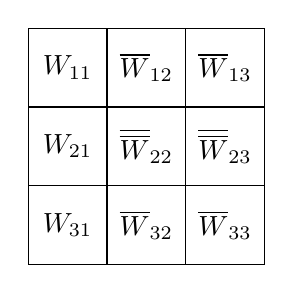
\begin{tikzpicture}[x=1cm,y=1cm]
      \draw (0,2) rectangle (1,3); \draw(0.5,2.5) node{$W_{11}$};
      \draw (1,2) rectangle (2,3); \draw(1.5,2.5) node{$\overline{W}_{12}$};
      \draw (2,2) rectangle (3,3); \draw(2.5,2.5) node{$\overline{W}_{13}$};
      \draw (0,1) rectangle (1,2); \draw(0.5,1.5) node{$W_{21}$};
      \draw (1,1) rectangle (2,2); \draw(1.5,1.5) node{$\overline{\overline{W}}_{22}$};
      \draw (2,1) rectangle (3,2); \draw(2.5,1.5) node{$\overline{\overline{W}}_{23}$};
      \draw (0,0) rectangle (1,1); \draw(0.5,0.5) node{$W_{31}$};
      \draw (1,0) rectangle (2,1); \draw(1.5,0.5) node{$\overline{W}_{32}$};
      \draw (2,0) rectangle (3,1); \draw(2.5,0.5) node{$\overline{W}_{33}$};
     \end{tikzpicture} }} \Punc{.}
  \end{align*}


\item \Xemph{Nulování submatic $\overline{\overline{W}}_{22}$ a $\overline{\overline{W}}_{23}$}

\item \Xemph{Doortogonalizace, totožná se zobecněnou ortogonalizací}

  \begin{align*}
    \tag{6.19}
    \vcenter{\hbox{
      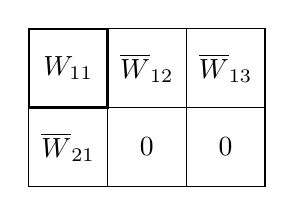
\begin{tikzpicture}[x=1cm,y=1cm]
    \draw[thick] (0,2) rectangle (1,3); \draw(0.5,2.5) node{$W_{11}$};
    \draw (1,2) rectangle (2,3); \draw(1.5,2.5) node{$\overline{W}_{12}$};
    \draw (2,2) rectangle (3,3); \draw(2.5,2.5) node{$\overline{W}_{13}$};
    \draw (0,1) rectangle (1,2); \draw(0.5,1.5) node{$\overline{W}_{21}$};
    \draw (1,1) rectangle (2,2); \draw(1.5,1.5) node{$0$};
    \draw (2,1) rectangle (3,2); \draw(2.5,1.5) node{$0$};
    \end{tikzpicture} }}
    \quad\longrightarrow\quad
    \vcenter{\hbox{
      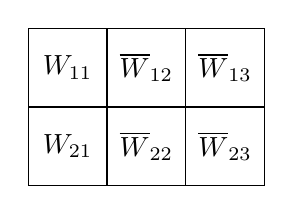
\begin{tikzpicture}[x=1cm,y=1cm]
      \draw (0,2) rectangle (1,3); \draw(0.5,2.5) node{$W_{11}$};
      \draw (1,2) rectangle (2,3); \draw(1.5,2.5) node{$\overline{W}_{12}$};
      \draw (2,2) rectangle (3,3); \draw(2.5,2.5) node{$\overline{W}_{13}$};
      \draw (0,1) rectangle (1,2); \draw(0.5,1.5) node{$W_{21}$};
      \draw (1,1) rectangle (2,2); \draw(1.5,1.5) node{${\overline{W}}_{22}$};
      \draw (2,1) rectangle (3,2); \draw(2.5,1.5) node{${\overline{W}}_{23}$};
     \end{tikzpicture} }} \Punc{,}
  \end{align*}

  \noindent
  \Xemph{kde \orig{59} submatice $W_{11}$ je základní, a kde proběhne
    pouze ortozonalizace pravé vedlejší submatice $[~0~~0~]$.}
  %
  Při ortogonalizaci
budou tedy od nulových sloupci pravé dolní submatice v (6.19)
odečítány lineární kombinace sloupců $W_{21}$ přičemž koeficienty
těchto lineárních kombinací se získají jako skalární součiny
sloupců odpovídajících horní (hlavní) submatici (viz (2.16) --
zobecněná ortogonalizace submatice $A_4$).

\item \Xemph{Zobecněná ortogonalizace}

  \begin{align*}
    \tag{6.20}
    \vcenter{\hbox{
      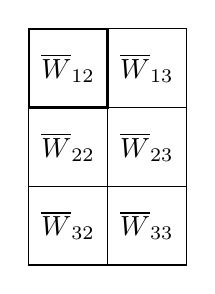
\begin{tikzpicture}[x=1cm,y=1cm]
      \draw[thick] (1,2) rectangle (2,3); \draw(1.5,2.5) node{$\overline{W}_{12}$};
      \draw (2,2) rectangle (3,3); \draw(2.5,2.5) node{$\overline{W}_{13}$};
      \draw (1,1) rectangle (2,2); \draw(1.5,1.5) node{$\overline{W}_{22}$};
      \draw (2,1) rectangle (3,2); \draw(2.5,1.5) node{$\overline{W}_{23}$};
      \draw (1,0) rectangle (2,1); \draw(1.5,0.5) node{$\overline{W}_{32}$};
      \draw (2,0) rectangle (3,1); \draw(2.5,0.5) node{$\overline{W}_{33}$};
    \end{tikzpicture} }}
    \quad\longrightarrow\quad
    \vcenter{\hbox{
      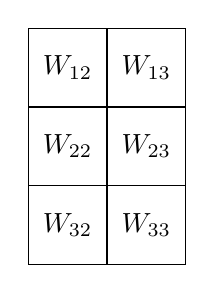
\begin{tikzpicture}[x=1cm,y=1cm]
      \draw (1,2) rectangle (2,3); \draw(1.5,2.5) node{$W_{12}$};
      \draw (2,2) rectangle (3,3); \draw(2.5,2.5) node{$W_{13}$};
      \draw (1,1) rectangle (2,2); \draw(1.5,1.5) node{$W_{22}$};
      \draw (2,1) rectangle (3,2); \draw(2.5,1.5) node{$W_{23}$};
      \draw (1,0) rectangle (2,1); \draw(1.5,0.5) node{$W_{32}$};
      \draw (2,0) rectangle (3,1); \draw(2.5,0.5) node{$W_{33}$};
     \end{tikzpicture} }}
  \end{align*}
  %
  \Xemph{se základní submaticí $\overline{W}_{12}$}.

  \noindent
  Shrneme-li, vidíme, že hledané submatice jsme určili zčásti při
  první ortogonalizaci v~prvním kroku a zčásti při třetí
  ortogonalizaci ve čtvrtém kroku algoritmu.


  Stejně jako u zobecněné ortogonalizace monou i u
  ortogonalizace algoritmem ORTON některé submatice v (6.17)
  chybět; naopak
  je možno směrem dolů a vpravo k~matici $A$ vhodné submatice
  připojovat. Je např. zřejmé, že budou-li chybět submatice
  $A_{11},A_{21},A_{31},A_{22}$ a $A_{34}$,
  bude se ORTON redukovat na zobecněnou ortogonalizaci matice
  %
  \begin{align*}
    \tag{6.21}
    \vcenter{\hbox{
      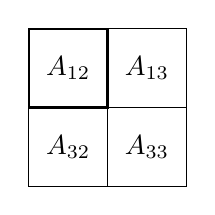
\begin{tikzpicture}[x=1cm,y=1cm]
      \draw[thick] (1,1)
                  rectangle (2,2); \draw(1.5,1.5) node{$A_{12}$};
      \draw (2,1) rectangle (3,2); \draw(2.5,1.5) node{$A_{13}$};
      \draw (1,0) rectangle (2,1); \draw(1.5,0.5) node{$A_{32}$};
      \draw (2,0) rectangle (3,1); \draw(2.5,0.5) node{$A_{33}$};
     \end{tikzpicture} }}     \Punc{,}
  \end{align*}
  %
  z čehož okamžitě plyne, že může být užit k vyrovnání
  zprostředkujících a podmínkových pozorování.
  Aplikace algoritmu k řešení úloh typu IC a CU probereme
  v následující kapitole.

\end{enumerate}

Základními \orig{60} prostředky, které nás vedly k formulaci
algoritmu ORTON, byl \name{SCHMIDŮV} princip extremálních vah a princip
doortogonalizace. Existují i jiné, přímější cesty odvození
stejného ortogonalizačníno postupu. Mohli bychom např. dokázat, že
k ORTONu vede i způsob řešení úlohy typu CU, založený na
eliminaci neznámých v jedné části podmínkových rovnic. Přesto jsme
dali přednost první cestě mj. proto, že nám umožnila dát nový
pohled na oba zmíněné princiny v širších souvislostech. Např.
doortogonalizačního principu může být užito nejen při řešení
úloh typu IC nebo CU, ale i při vyrovnání zprostředkujících
nebo podmínkových pozorování. Podle obou vět uvedených v tomto
odstavci je zřejmé, že i v takovém případě může doortogonalizace
zpřesnit výsledky \name{GRAMOVY-SCHMIDTOVY} ortogonalizace.


Podaná definice algoritmu ORTON shrnuje pouze základní
pravidla, na nichž je založen. Při realizaci v programu pro
počítač je třeba navíc výběrem sloupců matice $A$ nebo jiným vhodným
opatřením zajistit, aby matice $A_{21}$ byla regulární, je třeba
předvídat a testovat případnou singularitu (lineární závislost
sloupců
%
$
\begin{bmatrix}
  A_{11} & A_{12} \\ A_{21} & A_{22}
\end{bmatrix}
$
%
) apod. Na druhé straně nemusí program provádět stanovené operace v
předepsaném členění do čtyř izolovaných etap. Program může být výhodně
organizován cyklicky tak, že v každém kroku kompletně zpracuje jeden
sloupec matice $A$.  Takového přístupu bylo např. užito v proceduře
ORTON3 sestavené v jazyce ALGOL při ověřování algoritmu na počítači
ELLIOTT 503.  Základní vlastnosti procedury popisujeme v~ kap. 12.

\Pozn{1} Ve větě 2 jsme dokázali, že doortogonalizací se eliminuje
jistá složka vektoru chyby $\varphi_i\,'$ tak, že zbývající chyba
$\varphi_i\,' = \varphi_{i2}$ leží v podprostoru tvořeném vektory
$w_i,w_{i+1},\dots,w_m$. Chyba $\varphi_i\,''$ byla přitom definována
jako rozdíl
%
\begin{align*}
  \tag{6.22}
  \varphi_i\,'' = \widetilde w_i\,'' -  \widetilde w_i
\end{align*}
%
doortogonalizací korigovaného vektoru $\widetilde w_i\,''$ a
teoreticky exaktního vektoru $\widetilde w_i$. Zkoumejme nyní velikost
chyby $\psi_i^{(N)}$ vektoru $\widetilde w_i\,'$, který vznikl
normalizací vektoru $w_i\,''$. O vektoru $\widetilde w_i\,''$
předpokládáme, že je nenulový.

Označme nejprve \orig{61}
%
\begin{align*}
  \tag{2.23}
  \psi_i\,' = \widetilde w_i\,'' - w_i
  = \psi_{i1} + \psi_{i2} \Punc{,}
\end{align*}
%
kde $\psi_{i1} = \beta_i w_i$ představuje ortogonální projekci vektoru
$\psi_i\,'$ na vektor $w_i$ a $\psi_{i2}$ je ortogonální projekce
téhož vektoru na podprostor tvořený vektory
$w_{i+1},w_{i+2},\dots,w_m$ (obr. 6.4).
%
\begin{center}
%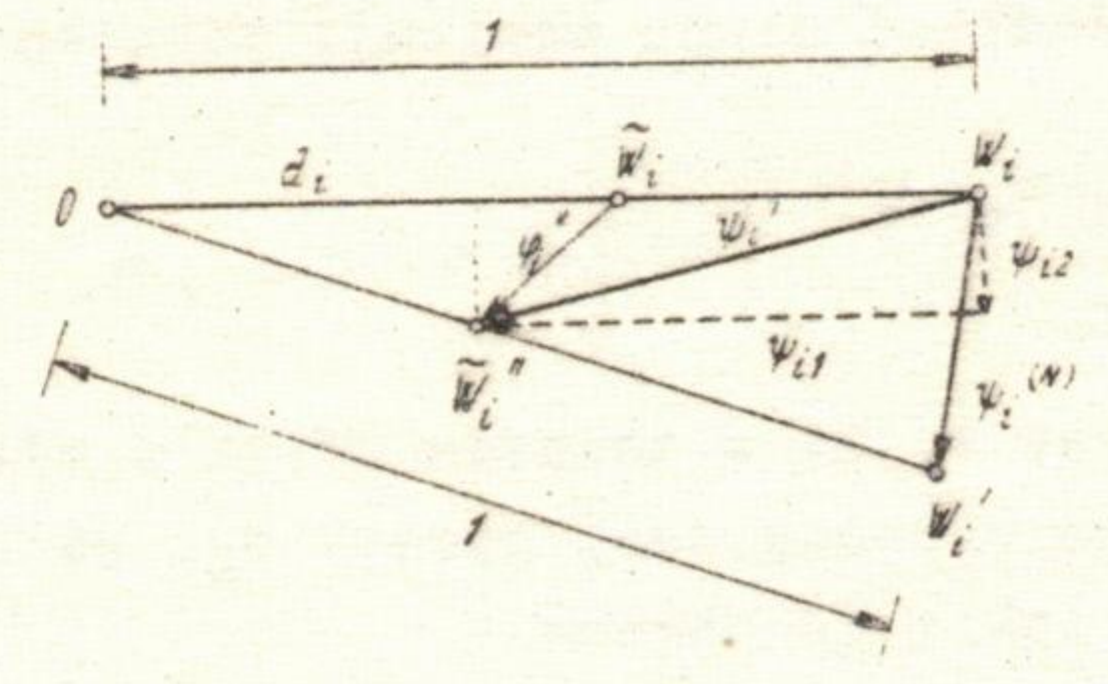
\includegraphics[width=0.5\textwidth]{obr_6.4.png}\\
% digitalizace https://yangcha.github.io/iview/iview.html
%
%\usetikzlibrary{calc}
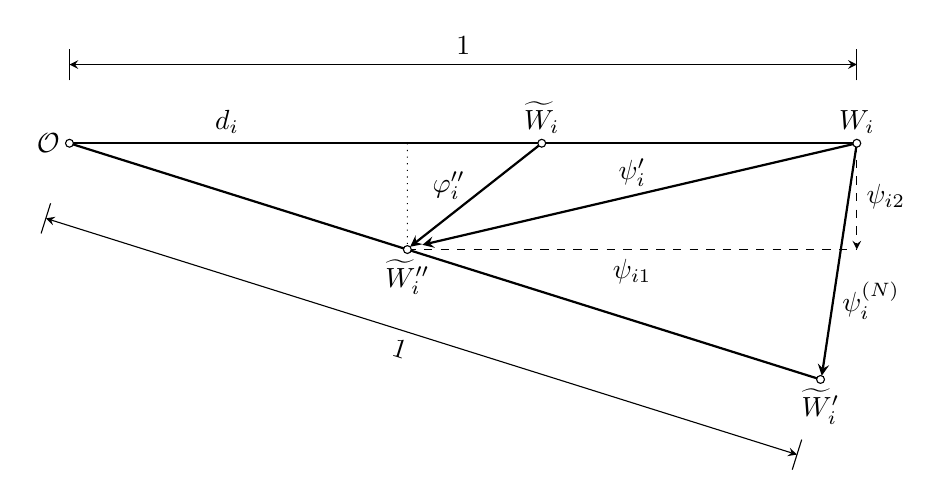
\begin{tikzpicture}[xscale=10,yscale=-10,>=stealth]
  \begin{scope}

    \def\dim{1.0000};            % dist unit
    \def\dc {0.0050};            % circle
    \def\cos{0.953939201416946}  % rotation 17.458 degrees
    \def\sin{0.300};

    \def\Ax{0};
    \def\Ay{0};
    \def\Bx{\dim};
    \def\By{0};
    \def\Fx{\dim*\cos};
    \def\Fy{\dim*\sin};
    \def\Cx{\dim/20*12};
    \def\Cy{\Ay};
    \def\Dx{\Fx/20.0*9};
    \def\Dy{\Fy/20.0*9}
    \def\Ex{\Bx};
    \def\Ey{\Dy};

    \coordinate (A) at (\Ax,\Ay);
    \coordinate (B) at (\Bx,\By);
    \coordinate (C) at (\Cx,\Cy);
    \coordinate (D) at (\Dx,\Dy);
    \coordinate (E) at (\Ex,\Ey);
    \coordinate (F) at (\Fx,\Fy);

    \begin{scope}
      \def\Gx{\Ax};
      \def\Gy{\Ay-0.1};
      \def\Hx{\Bx};
      \def\Hy{\By-0.1};
      \def\Kx{\Ax-0.1*\sin};
      \def\Ky{\Ay+0.1*\cos};
      \def\Lx{\Fx-0.1*\sin};
      \def\Ly{\Fy+0.1*\cos};

      \coordinate (G) at (\Gx,\Gy);
      \coordinate (H) at (\Hx,\Hy);
      \coordinate (K) at (\Kx,\Ky);
      \coordinate (L) at (\Lx,\Ly);

      \def\t{0.02}
      \draw[<->] (G)--(H);
      \draw[thin] (\Gx,\Gy+\t)--(\Gx,\Gy-\t);
      \draw[thin] (\Hx,\Hy+\t)--(\Hx,\Hy-\t);
      \node[above] at ({(\Gx+\Hx)/2},\Gy) {1};

      \draw[<->] (K)--(L);
      \draw[thin] (\Kx-\t*\sin,\Ky+\t*\cos)--(\Kx+\t*\sin,\Ky-\t*\cos);
      \draw[thin] (\Lx-\t*\sin,\Ly+\t*\cos)--(\Lx+\t*\sin,\Ly-\t*\cos);
      \node[below left,rotate=-17.458] at ({(\Kx+\Lx)/2},{(\Ky+\Ly)/2}) {1};
    \end{scope}

    \draw[thick] (A)--(B);
    \draw[thick] (A)--(F);

    \draw[thick, ->] (B)--(\Fx+\sin*\dc,\Fy-\cos*\dc);

    \draw[dashed, thin, ->] (B)--(E);
    \draw[thick, ->] (C)--(\Dx+0.707*\dc,\Dy-0.707*\dc);  % 0.707.. ~ sin(45)
    \draw[dashed, thin] (D)--(E);
    \draw[dotted] (\Dx,\Ay)--(D);
    \draw[thick, ->] (B)--(\Dx+\cos*4*\dc,\Dy-\sin*4*\dc);

    \draw[fill=white] (A) circle (\dc);
    \draw[fill=white] (B) circle (\dc);
    \draw[fill=white] (C) circle (\dc);
    \draw[fill=white] (D) circle (\dc);
    \draw[fill=white] (F) circle (\dc);

    \node[left]  at (A) {$\mathcal O$};
    \node[above] at (B) {$W_i$};
    \node[above] at (C) {$\widetilde W_i$};
    \node[below] at (D) {$\widetilde W_i''$};
    \node[below] at (F) {$\widetilde W_i'$};

    \node[above] at (0.2*\Bx,\Ay) {$d_i$};
    \node[left]  at ({(\Dx+\Cx)/2},{\Dy*0.40+\Cy*0.60}) {$\varphi_i''$};
    \node[above] at ({(\Dx+\Bx)/2},{(\Dy+\By)/2}) {$\psi_i'$};
    \node[below] at ({(\Dx+\Ex)/2},\Ey) {$\psi_{i1}$};
    \node[right] at (\Ex,{(\By+\Ey)/2}) {$\psi_{i2}$};
    \node[right] at ({(2*\Fx+\Bx)/3},{(2*\Fy+\By)/3}) {$\psi_i^{(N)}$};

  \end{scope}
\end{tikzpicture}

%

Obr. 6.4
\end{center}
%
Hledanou chybu $\psi_i^{(N)}$ určíme z rovnice
%
\begin{align*}
  \tag{6.24}
  \psi_i^{(N)}
    = \frac{\widetilde w_i\,''}{\Vert\widetilde w_i\,''\Vert} - w_i \Punc{.}
\end{align*}
%
Platí
%
\begin{align*}
  \tag{6.25}
  &\widetilde w_i\,'' = w_i + \psi_{i1} + \psi_{i2}
  = (1 + \beta_i)w_i + \psi_{i2} \Punc{,} \\
  \tag{6.26}
  &\Vert\widetilde w_i\,''\Vert^2 = (1 + \beta_i)^2 + \Vert\psi_{i2} \Vert^2 \Punc{.}
\end{align*}
%
Označíme-li $d_i = |1 + \beta_i|$ délku vektoru $(w_i + \psi_{i1})$,
dostaneme dosazením ze (6.25)a (6.26) do (6.24)
%
\begin{align*}
  \tag{6.27}
  \psi_i^{(N)} &=
  \left\{ d_i^2 + \Vert \psi_{i2} \Vert^2 \right\}^{-{1\over2}}
  \left\{(1 + \beta_i)w_i + \psi_{i2} \right\} - w_i = \\
  &= d_i^{-1} \left\{ 1 + (\Vert\psi_{i2}\Vert/d_i) \right\}^{-{1\over2}}
  \left\{(1+\beta_i)w_i + \psi_{i2} \right\} - w_i \Punc{.}
\end{align*}
%
Předpokládejme, že $(1+\beta_i) > 0$. Protože poměr $\Vert \psi_{i2}
\Vert/d_i$ bude zpravidla dostatečně malý, můžeme psát
%
\begin{align*}
  \tag{6.28}
  \psi_i^{(N)}\approx
  (w_i + \psi_{i2}/d_i)
  \left\{1 - {1\over2}(\Vert\psi_{i2}\Vert/d_i)^2\right\} - w_i
  \approx \psi_{i2}/d_i \Punc{,}
\end{align*}
%
se \orig{62} zanedbáním veličin řádu $(\Vert\psi_{i2}\Vert/d_i)^2$ a
menších. Chyba normalizovaného vektoru tedy prakticky leží v
podprostoru vektorů $w_{i+i},w_{i+2},\dots,w_m$ Projekce chyby
nenormalizovaného vektoru na vektor $w_i$ byla normalizací z větší
části eliminována.

\Pozn{2} Upozorníme ještě na souvislost principu doortogonalizace se
známou metodou pro zpřesnění výsledků řešení jedné kategorie úloh
při vyrovnání zprostředkujících pozorování.  Předpokládejme, že
vyrovnávací úlohu popisují rovnice oprav
%
% nedokažu vnutit i=1,2,...,m za složenou pravou zavorku }
\begin{align*}
  \tag{6.29}  v_i   &= \sum_{j=1}^{n} a_{ij} x_j + l_i \qquad  i=1,2,\dots,m \\
  \tag{6.30}  a_{i1} &= 1
\end{align*}
%
Je zřejmé, že součet oprav $v_i$ by v takovém případě měl být
nulový. Výsledkem numerického výpočtu jsou opravy $v+i\,'$ zatížené
zaokrouhlovacími chybami, takže je obecně
%
\begin{align*}
  \tag{6.31}  \sum v_i\,' \ne 0 \Punc{.}
\end{align*}
%
Opravy $v_i\,'$ je možno korigovat podle vzorce
%
\begin{align*}
  \tag{6.32} v_i\,'' = v_i\,' - \sum v_i\,'/m  \Punc{,}
\end{align*}
%
který odpovídá analogické korekci první neznámé
%
\begin{align*}
\tag{6.33}   x_1\,'' = x_1\,' - \sum v_i\,' / m \Punc{.}
\end{align*}
%
Touto jednoduchou úpravou dosáhneme nejen splnění podmínky $\sum
v_i\,'' = 0$, ale především zpřesníme řešení ve smyslu poklesu
součtu čtverců oprav. Za předpokladu (6.31) je totiž
%
\begin{align*}
  \tag{6.34}
  \sum (v_i\,'')^2 = \sum (v_i\,')^2
  -2(\sum v_i\,')^2/m + (\sum v_i\,')^2/m
  = \sum (v_i\,')^2 -(\sum v_i\,')^2/m < \sum(v_i\,')^2 \Punc{.}
\end{align*}
%
Dokážeme nyní, že výpočet oprav $v_i\,''$ podle (6.32) je ekvivalentní
doortogonalizaci vektoru $v'$ k prvnímu sloupci $w_1$ matice $W$,
vzniklé ortogonalizací matice soustavy (6.29). Označíme-li $a_1$
vektor tvořený koeficienty rovnic oprav $a_{i1}$ (6.30), bude podle
($2.1_1$) v důsledku vlastnosti (6.30)
%
\begin{align*}
  \tag{6.35}
  w_1 = a_1/\Vert a_1\Vert = m^{-{1\over2}}a \Punc{.}
\end{align*}
%
Na základě (6.6) proběhne doortogonalizace vektoru $v'$ k vektoru
$w_1$ takto \orig{63}
%
\begin{align*}
  \tag{6.36}
  v\,'' = v\,' - (v\,',w_1)w_1 = v\,' - m^{-{1\over2}}(\sum v_i\,')w_1
  = v\,' - m^{-1}(\sum v_i\,')a \Punc{.}
\end{align*}
%
Je tedy v souladu se (6.32)
%
\begin{align*}
  \tag{6.37}
  v_i\,'' = v_i\,' - \sum v_i\,'/m \Punc{.}
\end{align*}
